\chapter{Conclusions}
\label{ch:conclusions}

The objective of this dissertation was to develop further methodology for the use of network analysis in investigating innovation ecosystems with a data-driven approach. Being data-driven asserts that it should be possible to collect and aggregate data from various heterogeneous sources in an computational fashion and that the overall analysis process can be automated. In short, the process should allow reproducible analysis. More specifically, three individual objectives were set for the dissertation. First, \ref{objective:empirical} was to contribute to the empirical body of knowledge on innovation ecosystems by running a series of investigations on the structural properties of innovation ecosystems of different levels of abstraction and complexity. Second, \ref{objective:ecosystemnetworks} was to develop guidelines for modeling, representing, and measuring innovation ecosystems as networks for their visual analytics. Third and most importantly, \ref{objective:processmodel} was to design a generic process model for data-driven visual analytics of innovation ecosystems as networks.

To reach these objectives, research was conducted in two complementing streams. First, a series of investigations on innovation ecosystems was implemented to gain knowledge on the structural properties of innovation ecosystems and, even more importantly, the ways that investigators and innovation ecosystem actors and stakeholders prefer to model the innovation ecosystems as networks. Second, a set of requirements were distilled from the investigations--serving as Action Design Research \citep{Sein2011ActionResearch} experiments--to support the design of the generic process model for data-driven visual analytics of innovation ecosystems as networks.

The main conclusion we draw from the investigations is that conducting data-driven investigations on innovation ecosystems with a network-centric mindset is a valid approach for mapping, exploring, and describing the structure of these ecosystems. Through a series of investigations, we show that innovation ecosystem investigators and even more importantly innovation ecosystem actors and other stakeholders find value in using network analytics in investigating and exploring their innovation ecosystems of interest. 

Addressing innovation ecosystems as networks enables scholars and practitioners to study their complexity and provides means for mapping, monitoring, and managing the individual actors in an innovation ecosystem under investigation. In this dissertation, we have presented experiments in taking a data-driven network analytics approach to investigate innovation ecosystems in platform, business domain, program, national, and international level. In all of the contexts, the main objective of the investigations eventually is to support innovation and growth. Following the Action Design Research approach, a design science variant that is based on iterative and incremental construction of artifacts, here network visualizations and supporting processes, has allowed us to collect constant feedback from the innovation ecosystem stakeholders through the process of guided emergence.

This dissertation contributes to the emerging field of data-driven innovation ecosystem research in three major ways. First, we contribute to the field of innovation ecosystem research with a series of empirical investigations on the structure and evolution of innovation ecosystems of different levels of abstraction and complexity. These investigations are described in Chapter~\ref{ch:experiments}. Second, through the individual investigations serving as Action Design Research experiments, we have developed and described design guidelines for representing and analyzing innovation ecosystems as networks. The guidelines are presented in Chapter~\ref{ch:ecosystemnetworks}. Third and most importantly, we have developed and began the validation of the Ostinato Model, a process model for data-driven visual network analytics of innovation ecosystems. The Ostinato Model, described in detail in Chapter~\ref{ch:ostinato}, is the key contribution and result of this dissertation.

The Ostinato Model has two main phases, Data Collection and Refinement and Network Creation and Analysis. The Data Collection and Refinement phase is divided into Entity Index Creation, Web/API Crawling, Scraping, and Data Aggregation. The Network Creation and Analysis phase is composed of Filtering in Entities, Node and Edge Creation, Metrics Calculation, Node and Edge Filtering, Entity Index Refinement, Layout Processing, and Visual Properties Configuration. Finally, the visualizations are provisioned to investigators and other end users with interactive exploration tools and discussion, and their feedback activates an iteration of the process. A cycle of exploration and automation characterizes the model and is embedded in each phase.

In addition to the Ostinato Model, we contribute with a set of design principles for investigating innovation ecosystems as the networks. The design principles we have identified support modeling, analyzing, and visualizing innovation ecosystems as networks, investigating network evolution, allowing for interactive network exploration and sharing the findings. 

Both the Ostinato Model and the design principles for investigating innovation ecosystems as networks were developed over multiple experiments following Action Design Research. Importantly, Action Design Research comes with inbuilt mechanisms supporting the validation of the created artifacts. The driving principle for validation is guided emergence through which artifacts are created in constant collaboration with actors and organizations to which the artifact is developed for. Moreover, the perpetual collaboration allows for authentic and concurrent evaluation, i.e. evaluation is not a separate step but takes places throughout the artifact creation process. As discussed in detail in Section~\ref{sec:evaluation}, we have applied authentic and concurrent evaluation in developing both of the key artifacts of the dissertation.

There are three primary target groups that will utility in the results of this dissertation.

First, capability to derive structural insights in ecosystem and actor level from data is imperative in pushing the academic research forward. A great majority of innovation ecosystem research takes place either in the level of individual organizations or pairs (dyads) of these organizations \citep{Jarvi2016TakingReview}. Outside of this dissertation, a limited amount of empirical research on innovation ecosystems exists. Key means for breaking the limitations of providing ecosystem-level insights into ecosystems implicit in name-generating surveys is the the utilization of archival records in sourcing data for computational analysis of innovation ecosystems \citep[cf.][]{Williams2015MixedAnalysis}. The Ostinato Model supports the utilization of new sources of digital data in research. Importantly, digital data is often transactional microdata, i.e. it represents timestamped actor-level interactions supporting structural analysis of innovation ecosystems. 

Second, the domain of computational innovation ecosystem analytics, an extension of business ecosystem analytics, benefits equally from the ecosystem-level views created with the Ostinato Model. Even more importantly, the Ostinato Model can be used to design and implement the architecture of analytical tools and dashboards that render views into innovation ecosystem structure in a self-service mode. The target users here include business actors that seek to facilitate the emergence of innovation ecosystems and orchestrate their evolution. 

Third, views into the structure and dynamics of an innovation ecosystem may potentially have a focal role in innovation ecosystem orchestration. Data-driven visualizations are an organic part of Innovation Ecosystem Transformation Framework (IETF) in which visualizations are utilized to support innovation ecosystem actors in arriving a shared vision of the future toward which they work following their individual paths. 

We have used a number of datasets in these investigations, including social media, socially constructed data available online, and proprietary sets of data represented as spreadsheets and other formats. The experiments included in this dissertation are built on two key main sources of data. Socially constructed and curated IEN Dataset, more specifically IEN Executives and Finance and IEN Angels and Startups, has served as the main source of data. IEN Dataset is used for data on startups and growth companies and their transactions with individuals, investors, and other innovation ecosystem actors. Moreover, Thomson Reuters SDC data was used for data on deals and alliances between already established enterprises. In addition, we have used Twitter data for mapping the customer landscape around Tekes Young Innovative Companies and Demola in-house data for data on innovation projects and their actors over time. Moreoveor, the Ostinato Model is designed to include the collection of new sets of digital data relevant for a particular investigation.

\section{Implications to innovation ecosystem actors} 

The research in this dissertation is conducted in close interaction with a number of innovation ecosystem actors and stakeholders. Innovation ecosystem investigators, i.e. the co-authors of the articles included in the dissertation, form the core group of co-creators. Moreover, through the investigations, we have interacted with innovation ecosystem orchestrators (EIT ICT Labs), policy makers (Tekes, Ministry of Employment and the Economy representatives, Council of Tampere Region) as well as startup entrepreneurs, investors, and other innovation ecosystem actors. Next, we will provide a set of implications that stem from the dissertation research.

\subsection{Innovation ecosystem investigators}

Innovation ecosystem is new research domain with limited amount of empirical research. Several novel streams of data are, however, available to be fed into analysis to extend the empirical body of knowledge on innovation ecosystems. The network-based approach comes with new metrics and the objective for creating a system-level view instead of a more atomistic, sample-through-survey-based way of conducting research. Developing the investigative process in an iterative and incremental manner is imperative in managing the complexity. Exploratory, interactive, and transparent analytics process supports  maintaining balanced communication between the members of the investigative team in a major way and therefore supports interdisciplinary collaboration. 

The key result of this dissertation work, the Ostinato Model for data-driven visual network analytics, will help innovation ecosystem investigators in designing data-processing pipelines and architectures for visual network analytics of innovation ecosystems. In order to be able to a) develop independent software components or b) integrate existing API-based services that excel in individual parts of the process, there has to be a clear distinction and structure in between individual steps of the process. We look forward to observe how innovation ecosystem investigators will make use of the Ostinato Model in seeking interoperability in developing components and toolchains for the data-driven visual network analytics process.

In addition to visual analytics, innovation ecosystem scholar will benefit from applying the Ostinato Model and design principles for analyzing innovation ecosystems as networks when creating network models of innovation ecosystems for quantitative and statistical analysis. As we have shown in this dissertation, a rich variety of options exists in data sources, network modeling decisions, selection of node and network level metrics and, crucially, boundary specification. All of these options will make a major difference in the metrics that are fed into statistical and machine learning models and therefore the creation process of the network model of an innovation ecosystem should be made as transparent and tractable as possible. 

Through a process following the Ostinato Model, innovation ecosystem analysts get an access to empirical data that can be fed to agent-based and other models of innovation ecosystems. This allows investigations on the impacts of the structure and conduct \citep{Afuah2013,Ahuja2012TheNetworks} of the innovation ecosystem of interest; networks represent the pathways that show where recent activity has taken place.

In all, quantitative and statistical analysts will find the ability to maintain low entry barrier and high transparency as well as automation and overall reproducibility as useful as those that investigate innovation ecosystems with visual analytics approach particularly useful in qualitative investigations.

\subsection{Innovation ecosystem orchestrators and policy makers}

In this section, for brevity, we use (innovation ecosystem) orchestrators to refer to policy makers, program developers, university and technology park actors, and others with a similar role in facilitating innovation activities that cross the boundaries of individual organizations.

Both from policy making and innovation ecosystem orchestration viewpoint, the key contribution of this dissertation is the provision of a system-level view for innovation ecosystems of interest in the investigative context. With the help of the design guidelines described in Section~\ref{sec:designguidelines} and the Ostinato Model, similar system-level views can be created to individual ecosystems of different levels of abstraction and complexity. Moreover, Innovation Ecosystem Transformation Framework \citep{Russell2011TransformingOrchestration, Russell2015RelationalEcosystems} provides a holistic way to organize the data-driven, evidence-based orchestration efforts in a rigorous manner.

\begin{figure}[htb]
\centering
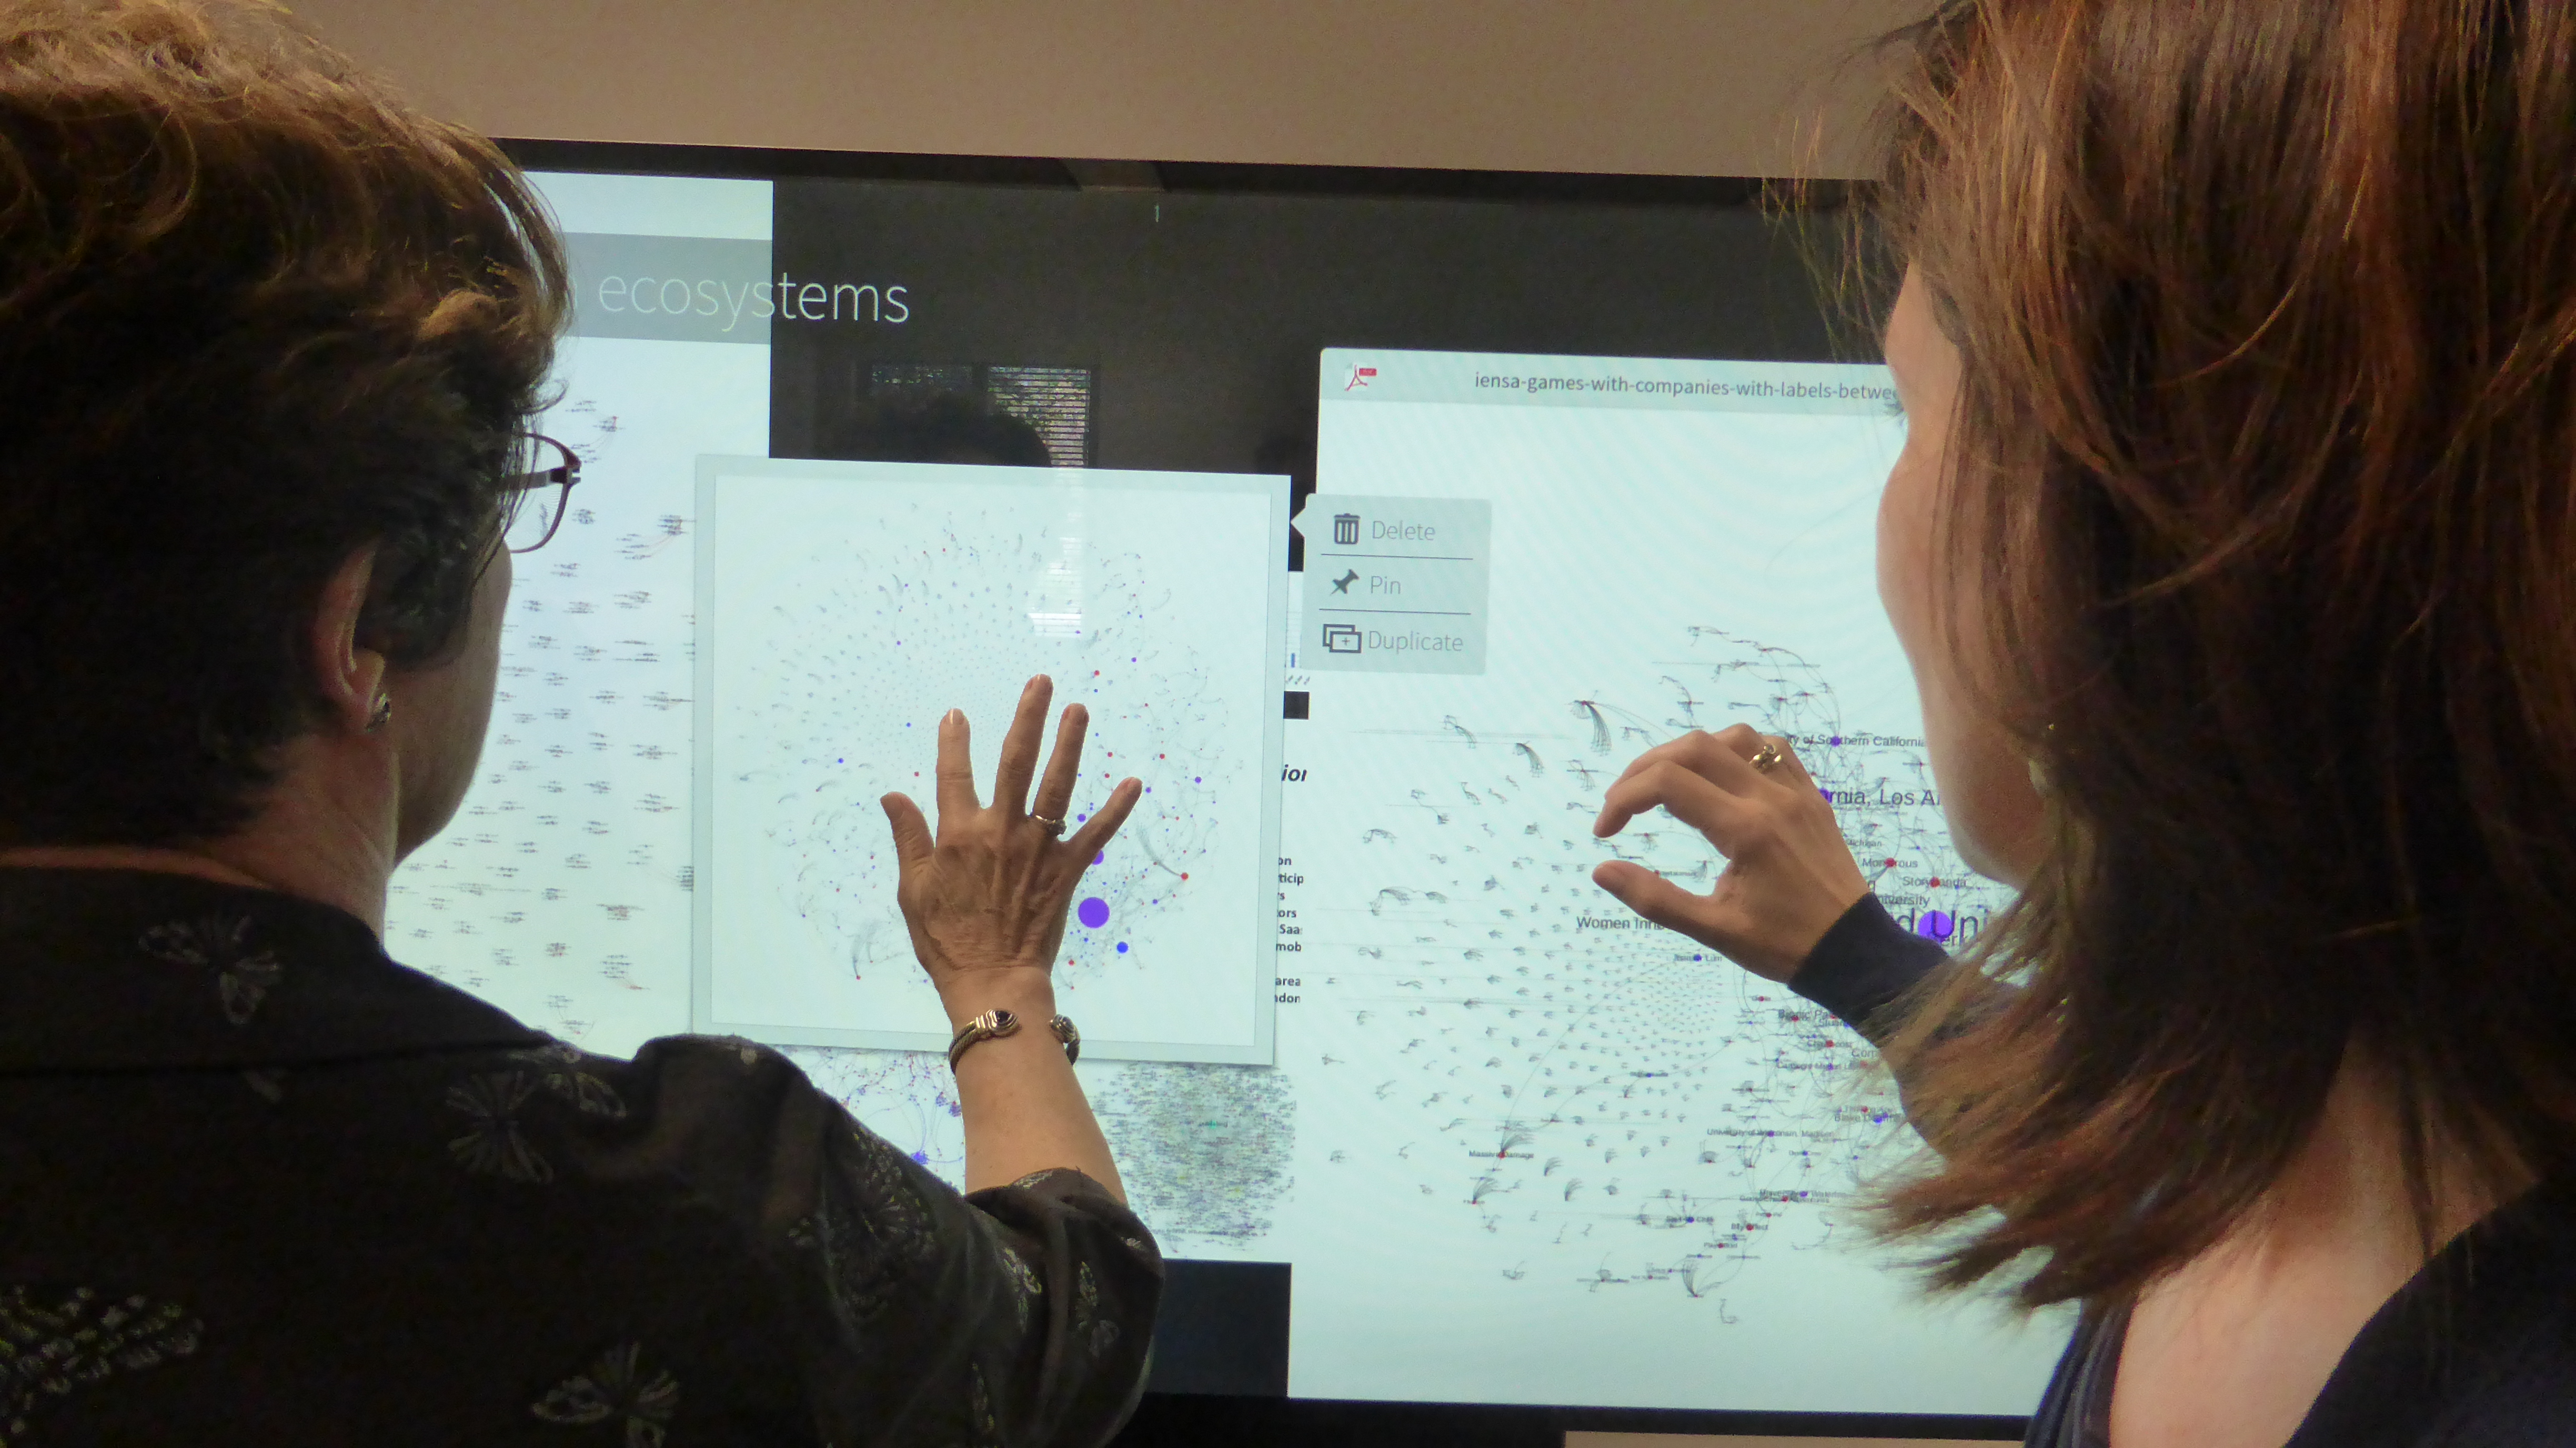
\includegraphics[width=13.5cm]{figure/interactive-visual-innovation-ecosystem-analytics.jpg}
\caption{New technology allows more interactive ways to explore data for sensemaking. Prototype visualization explored using \href{https://www.bluescape.com/}{Bluescape} on \href{http://www.multitaction.com/}{MultiTaction}.}
\label{fig:interactiveanalytics}
\end{figure}

\begin{figure}[htb]
\centering
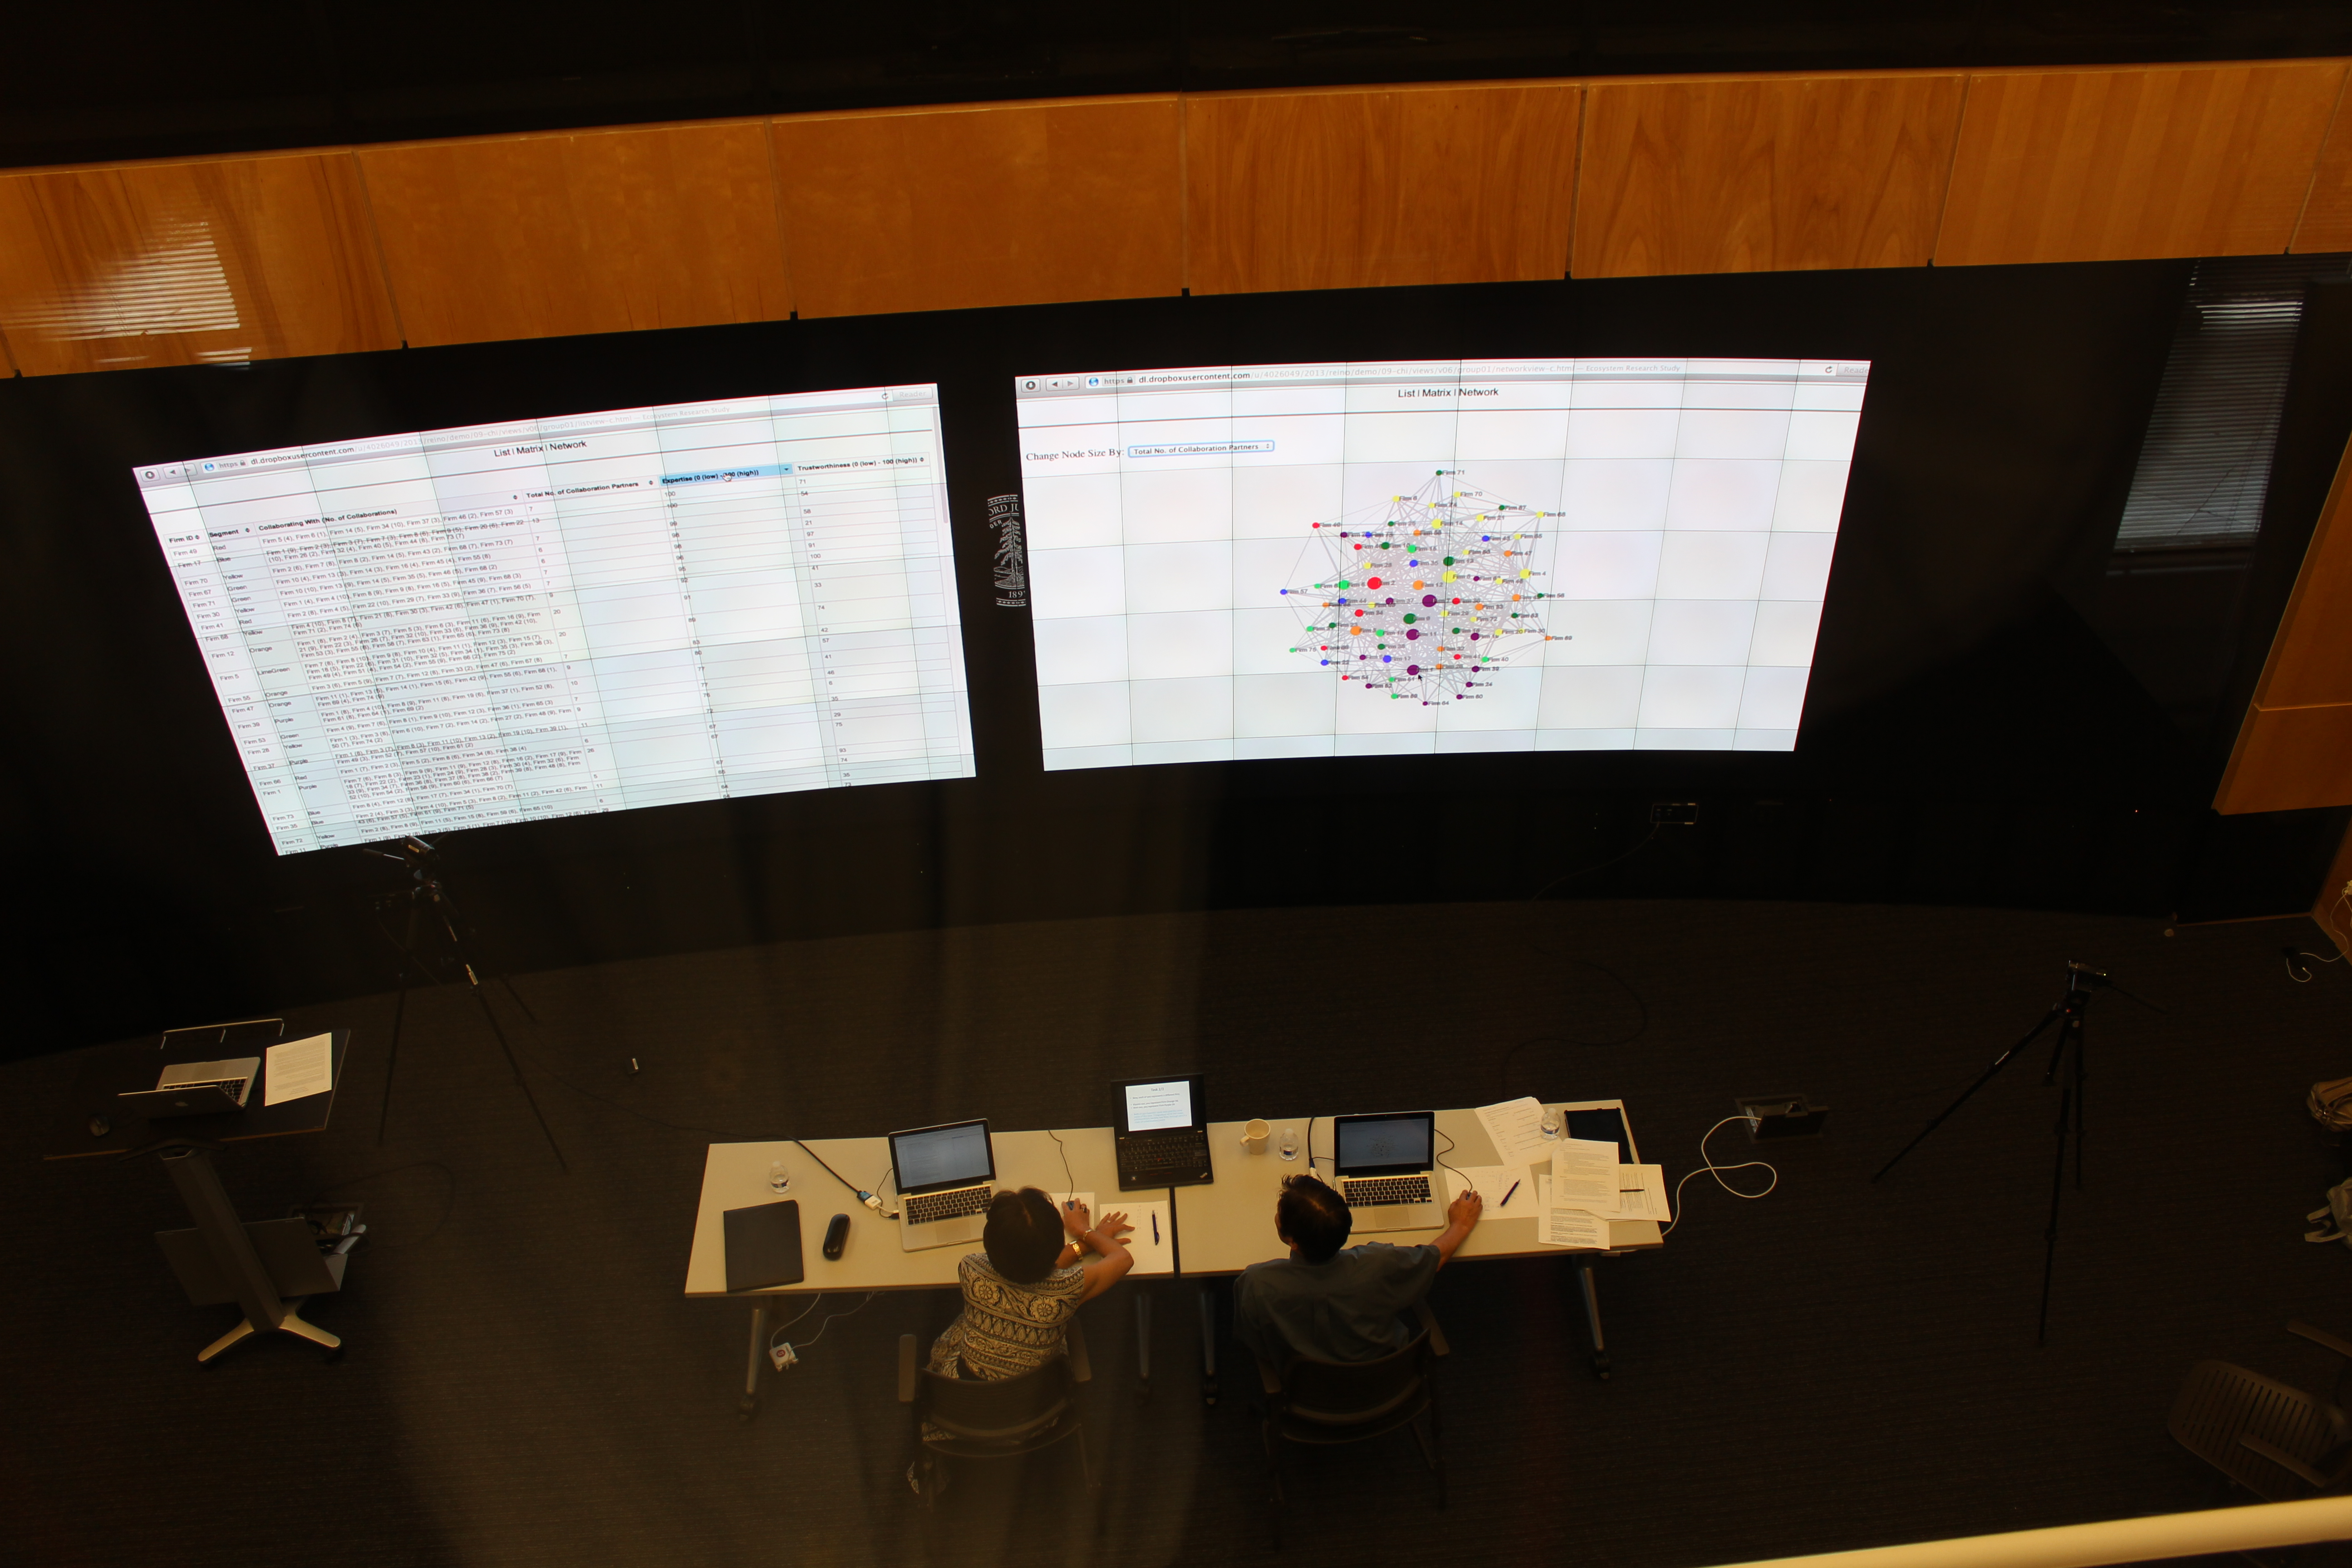
\includegraphics[width=13.5cm]{figure/decision-making-experiment.jpg}
\caption{Visual analytics supporting decision-making. Experimental setting at Stanford in 2013.}
\label{fig:experiment}
\end{figure}

We do not propose replacing the traditional statistical indicators with the system level view. Instead, we claim that the system-level view does support holistic insights of the innovation ecosystem structure and evolution and, moreover, give context to individual indicators and measurements. There is, however, a mismatch between the existing statistics available for orchestrators and the objective to the creation of a system-level view. Statistics are often if not in most cases aggregated into categories e.g. according to classification of economic activities\footnote{Toimialaluokitus in Finnish.} For creating a system-level view, transactional microdata is needed, i.e. long form data that represents the individual actor-level transactions over time.

Data on scientific articles is a good example of transactional micro-level relational data. The authors of the articles are enumerated and date information is available. Moreover, the authors whose work has provided the knowledge baseline for the article are explicitly mentioned through citations. The availability of bibliographic data as well as its relative importance and the fact that is is well-known to reseachers. This has led to a significant body of literature on the bibliometrics and scientometrics. At the same time, accessing and particularly aggregating bibliometrical data from multiple sources continues to be far from trivial. Data formats vary and global identifiers for actors do now exist in the data.

We urge orchestrators not to settle with data that is aggregated through a static, lagging-behind taxonomy. These taxonomies are great for long-term, consistent, comparable statistics and statistical analysis. For action-oriented, real-time, policy making, learning what is working and therefore providing a constantly improving environment for ecosystemic innovation activities is a key priority. Therefore, orchestrators should make sure that they have access to multi-level temporal data on companies, their creators and enablers--including venture-capital investors--in a way that enables the creation of multiscopic views of the ecosystem. Moreover, orchestrators should at least consider providing access to this data to those that are interested. Steps toward this direction are taken at the moment: dataset on projects funded by both Academy of Finland, Tekes as well as European Commissions Horizon 2020 are available online. Work remains to be done even among the aforementioned examples, particularly to make sure that the features that are expected from open data are met.\footnote{According to \href{Open Knowledge}{https://okfn.org/opendata/}, ``‘Open knowledge’ is any content, information or data that people are free to use, re-use and redistribute — without any legal, technological or social restriction.''} Organizations leading the digital transformation, e.g. Cap Digital\footnote{Cap Digital: the French business cluster for digital transformation, \url{http://www.capdigital.com/}}, apply extensively the data-driven approach in developing and orchestrating their innovation ecosystem.

Finally, we encourage the orchestrators to make use of the new interactive tools in making sense of innovation ecosystems of their interest. Figure~\ref{fig:interactiveanalytics} gives an example of a setup based on a large touchscreen allowing for co-exploration and co-referencing. A bolder vision for supporting evidence-based decision making for innovation ecosystem orchestration would be to build a situation room, physical or virtual, with a visual representation supporting situation awareness\footnote{Tilannekuva in Finnish.}. Figure~\ref{fig:experiment} shows an example of a possible setup. Those who take up visual analytics should, however, bear in mind that while visualizations support users in making faster decisions, the confidence that actors have about their decisions does not predict the accuracy of the decisions. Therefore, it is important to validate the usefulness of the visual tools developed to support decision-making trough user experiments.

\subsection{Other ecosystem actors: startups, enterprises, investors}

We acknowledge that in socially constructed data, there is very likely a significant bias toward startups, incubators, and programs in which participants invest into communicating about their activities, the funding rounds they receive, the advisers that support the creation and development of the companies, perhaps even the versions of products being built. At the same time, we want to note that such a bias may very likely exist in the field of innovation in general, particularly in context of consumer products and services-–those that use effort for communicating about their results will, in general, be more likely to be successful and make a more significant impact. In scientific publishing, for example, those that communicate about their results and publications will receive more attention and are likely to receive more citations and therefore get better marks in citation-based measurements including h-index \citep[cf.][]{Terras2012}. 

In order to enable visibility and draw attention, a startup should make sure that they have a presence in different social media platforms as well as community-curated databases including Wikipedia, CrunchBase and others. The startups should have a website with latest information on the team, advisors, investors, references, and other connections of significance. 

Using navigation in the physical world as a metaphor, the approach presented in this dissertation does introduce means to draw maps of the structure or the topology of innovation ecosystems. When presenting the approach and results of the investigations included in this dissertation to startup ecosystem actors, they note the value of real-time maps of innovation ecosystem in keeping up with the evolution of the ecosystem--their competitors, developers of complementary products and services. Network maps give context to information on individual companies, e.g. the way a particular product or service is described.

\section{Limitations}

Key limitation in the presented Ostinato Model is the volume of data in use in the investigation. More specifically, while the Ostinato Model per se can be used to structure a process that is built e.g. with Apache Spark\footnote{Apache Spark - Lightning-fast cluster computing, \url{http://spark.apache.org/}} or Hadoop, the use of static (tabular) files in representing data adding to the transparency of the process to non-technical investigators becomes impossible once the volume of the data increases to a certain limit. However, while the source data may be voluminous, Entity Index Creation, Node and Edge Filtering and boundary specification all provide means to manage the amount of data in the investigative process.

Big data, computational social science and visual analytics are all fields that receive justified criticism \citep[cf.][]{boyd2012CriticalData}. We acknowledge that a series of investigations both in laboratories as well as in the wild have to be conducted to validate and refine the ways data-driven visual analytics best serves to supporting cross-organizational innovation activities and therefore in making world a better place.

\section{Future work}

This dissertation opens up several venues for additional research. Future work includes, first, the refinement of the Ostinato Model on basis of the feedback collected from researchers and practitioners working with the exploration–automation cycle of data-driven visual network analytics and applying the model.

Second, to lower the barrier for applying the Ostinato Model in supporting data-driven investigations and orchestration of innovation ecosystems, a software framework following the Ostinato Model should be implemented. At best, the framework would allow easy access (Web-based), real-time operations (stream-based processing). Moreover, the practices of both contemporary software development and interactive computing should be taken into account when developing such a framework. Practices related to existing tools such as Grunt\footnote{Grunt: The JavaScript Task Runner, \url{http://gruntjs.com/}}, a popular Javascript-based task runner as well as Python-based automation tools including PyBuilder\footnote{PyBuilder: Build automation for Python, \url{http://pybuilder.github.io/}}\footnote{Cf. related discussion on Twitter, \url{https://twitter.com/jsalonen/status/612644821052878848}} and Luigi\footnote{Luigi: build complex pipelines of batch jobs in Python, \url{https://github.com/spotify/luigi}} should be investigated for best practices.

We claim that that the Ostinato Model is general enough to be used in domains outside innovation ecosystem studies. In fact, we have already taken steps toward generalizing and validating the Ostinato Model in investigations outside the sphere of innovation ecosystem studies. The author of the dissertation has already joined with other investigators to apply the Ostinato Model case studies additional to the ones included in this dissertation. This work includes both innovation ecosystem analysis \citep{Russell2015RelationalEcosystems}, investigations of the use of Twitter in emerging communities \citep{Aramo-Immonen2015ExploringData,Jussila2014,Aramo-Immonen2016VisualizingModel} as well as in communication between political and journalistic elite 
\citep{Ruoho2015,Vainikka2015TviittienTwitterissa}. More experience on the use of the Ostinato Model, in particular by investigators other than the author of this dissertation, is needed to evaluate the true value and generalization potential of the Ostinato Model.

As an ecosystem of tools and components develops and requirements for interoperability are articulated, we see the possibility of developing a community of people moving the field forward. They will need a package management framework, system components, and a supportive community. We look forward to contributing to this work.